\documentclass[11pt,a4paper]{article}

\usepackage[T1]{fontenc}
\usepackage[utf8]{inputenc}
\usepackage[margin=2.4cm]{geometry}
\usepackage{graphicx}
\usepackage{amsmath,amssymb}
\usepackage{bm}
\usepackage{hyperref}
\usepackage{xcolor}
\usepackage{siunitx}
\usepackage{booktabs}
\usepackage{natbib}
\usepackage{caption}
% Cross-reference the main manuscript (e.g. Eq.~(b)); needs
% manuscript.aux, so compile the main file first (the Makefile does).
\usepackage{xr-hyper}
\externaldocument{manuscript}

\captionsetup{font=small,labelfont=bf,labelsep=period,justification=raggedright,singlelinecheck=false}

\hypersetup{colorlinks=true, linkcolor=blue!50!black, citecolor=blue!50!black, urlcolor=blue!50!black}

\graphicspath{{../figures/}}

% S-numbering for supplementary figures and tables.
\renewcommand{\thefigure}{S\arabic{figure}}
\renewcommand{\thetable}{S\arabic{table}}
\renewcommand{\theequation}{S\arabic{equation}}

\begin{document}

\title{Supplementary Material\\[0.4em]
\large A two-feedback Vicsek--Couzin flock: density-stratified heading
correlations as the robust fingerprint of motility--noise coupling}

\author{Yaya Youssouf Yaya}

\date{\today}

\maketitle

\subsection*{Order-parameter distribution at $L = 30$}

The Binder dip is ambiguous on its own: a weakly first-order
transition deepens $U_4$ through a bimodal
$P(\langle\varphi\rangle)$, while a continuous transition with
large $\gamma/\nu$ deepens it without bimodality. Only the
full distribution separates the two. We histogram
$\langle\varphi\rangle$ on long trajectories at $L = 30$,
$N = 2000$, three seeds, $6000$ measurement steps each, for
the motility-only ablation at $\eta = 0.10$ and the
double-adaptive model at $\eta = 0.15$
(Fig.~\ref{fig:transition}a). Both histograms come out unimodal.

\begin{figure}[htbp]
    \centering
    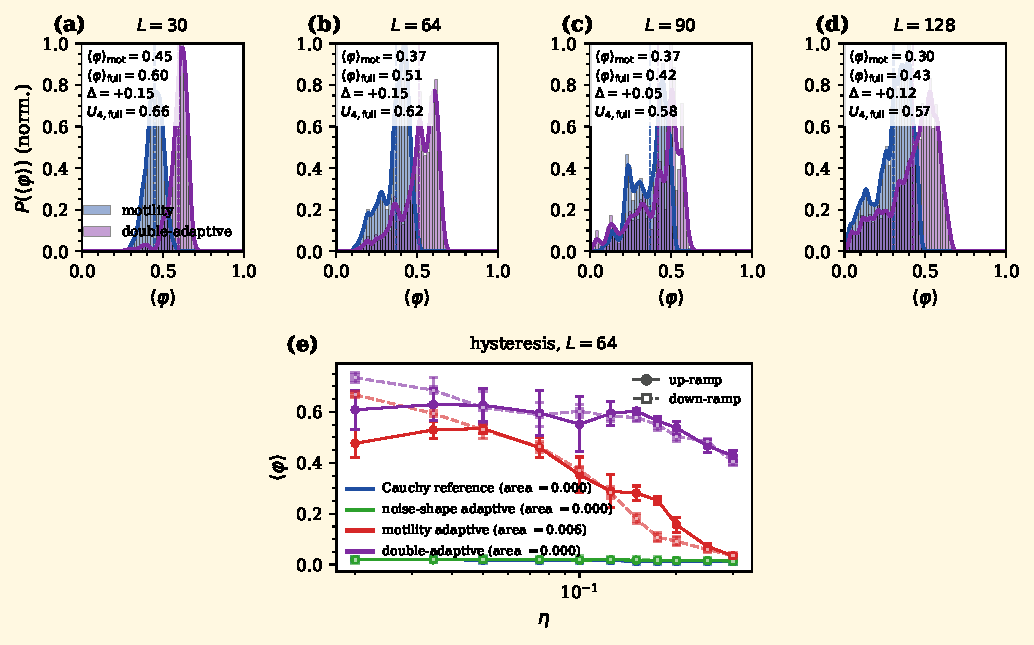
\includegraphics[width=\linewidth]{fig_double_transition.pdf}
    \caption{Order of the transition. (a)--(d)
    order-parameter distribution $P(\langle\varphi\rangle)$ with
    motility-only and double-adaptive overlaid, one panel per size
    (a) $L = 30$, (b) $L = 64$, (c) $L = 90$, (d) $L = 128$ (motility
    at $\eta = 0.10$, double-adaptive at $\eta = 0.15$), each
    normalised to its own peak and sharing the vertical scale; dashed
    lines mark the per-mode means and each panel reports the mean gap
    $\Delta$ and the full-mode Binder cumulant $U_4$. (e)
    quasi-static $\eta$ ramp up (filled circles, solid) and down
    (open squares, dashed) at $L = 64$, five seeds, the two
    motility-active modes (hue), with the loop areas. $P(\langle\varphi\rangle)$ stays
    single-peaked at every size and the hysteresis loops are
    negligible ($\leq 0.006$): the deepened Binder dip is not a
    coexistence signature and the transition is continuous (at most
    very weakly first-order).}
    \label{fig:transition}
\end{figure}

Motility-only peaks at $\langle\varphi\rangle \simeq 0.45$
with skewness $-0.25$, kurtosis $-0.14$ (a mildly left-skewed
broad mode); the double-adaptive model peaks at $0.60$ with
a sharper core (kurtosis $+5.56$) and a long left tail
(skewness $-1.88$). The long-trajectory Binder cumulants
$U_4 = 0.65$ (motility) and $0.66$ (full) sit just below the
bimodal limit $U_4 \to 2/3$ and well above the Gaussian
$U_4 = 0$: the trajectories are locked in a single ordered
state with bounded fluctuations, not switching between two
phases. The transition is at most weakly first-order here.

Rerunning the histograms at $L = 64, 90$ (five seeds,
$6\,000$ steps) and at $L = 128$ (five seeds, $60\,000$
steps) in panels (b)--(d), the double-adaptive distribution
sits to the right of motility-only at every size:
$\Delta\langle\varphi\rangle = +0.145, +0.048, +0.121$ at
$L = 64, 90, 128$ (the $L = 90$ row a seed-budget outlier
already seen in $s_{\rm sep}$). The full-mode $U_4$ stays in
$[0.57, 0.62]$ and the distributions broaden into mildly
platykurtic shapes at $L = 128$ ($\kappa = -0.27$ for
motility, $-0.20$ for full) without developing two-peak
structure. $P(\langle\varphi\rangle)$ remains unimodal across
all four sizes.

\subsection*{Hysteresis across the transition}
\label{sec:hysteresis}

The unimodal $P(\langle\varphi\rangle)$ and the ambiguous
$U_4$ dip leave the order of the transition unsettled; a
hysteresis test settles it. We ramp $\eta$ quasi-statically
up and back down at $L = 64$, five seeds, carrying the
configuration over from one step to the next (no
re-randomisation), for the two motility-active modes
(Fig.~\ref{fig:transition}e). The up- and down-ramp
$\varphi(\eta)$ branches overlap within error bars and the
loop area is negligible: $0.006$ for motility-only,
$0.000$ for the double-adaptive model. A first-order
transition would open a finite loop; its absence, with the
unimodal $P(\langle\varphi\rangle)$, places the transition in
the continuous (or at most very weakly first-order) class.

\subsection*{Time-averaged density profile along the polar axis}

The dense phase still has to be characterised geometrically:
does it travel as a metric-Vicsek soliton or sit as an
isotropic patch comoving with the flow? The band-soliton
index $b$ of Eq.~\eqref{eq:b} discriminates
($b \gtrsim 1.5$ for a band, $b \simeq 1$ for a patch). We
measure $b$ for all four heavy-tailed modes at their
near-critical $\eta$, $L = 30$, three seeds, $4000$
measurement steps (Fig.~\ref{fig:profile}).

\begin{figure}[htbp]
    \centering
    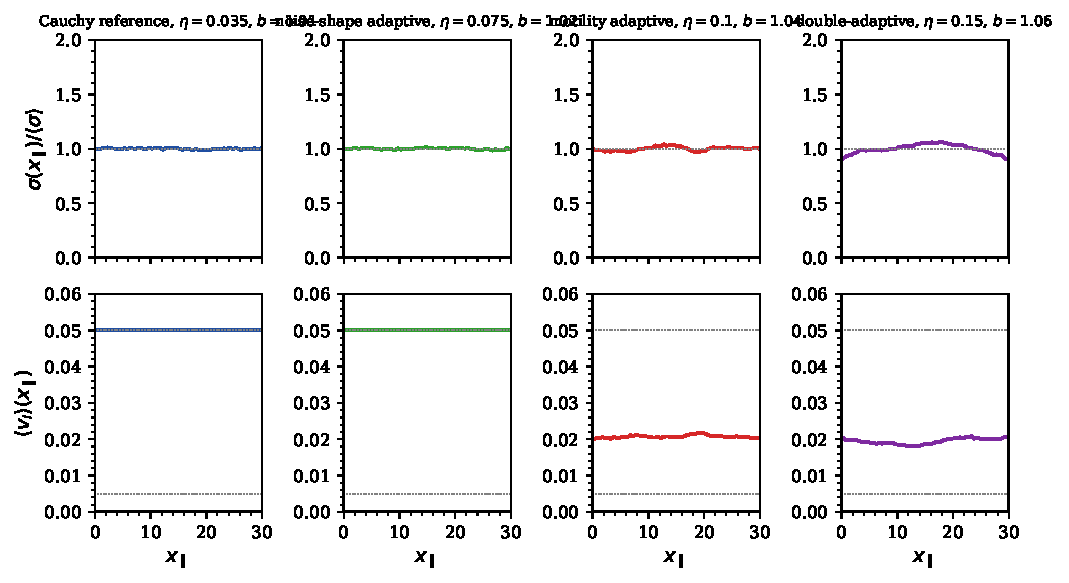
\includegraphics[width=0.95\linewidth]{fig_double_profile.pdf}
    \caption{Time-averaged profiles along the instantaneous
    polar-flow axis $x_\parallel$ at $L = 30$, three seeds,
    $4000$ measurement steps, the four modes overlaid at
    their respective near-critical $\eta$. (a) density
    normalised to its peak, with the band-soliton index $b$ per
    mode in the legend. (b) local speed normalised to its
    peak. Every profile is flat ($b \simeq 1$), so the
    motility-built dense phase is an isotropic comoving patch, not a
    travelling Vicsek band.}
    \label{fig:profile}
\end{figure}

All four profiles are flat to within $7\,\%$ ($b = 1.01,
1.02, 1.04, 1.06$ in the order Cauchy, noise-shape, motility,
full). None supports a metric-Vicsek band: the motility-built
dense phase either reorganises faster
than its polar axis or is isotropic in the comoving frame.
The full mode is marginally the most cohesive, consistent
with the Gaussian rectification tightening the patch from
within, but the increment is well below the soliton
threshold.

\subsection*{Why $\chi_{\max}(L)$ is a crossover, not an exponent}

The log--log slopes $a_{\rm motility} = +1.04$ and
$a_{\rm full} = +1.49$ of Table~\ref{tab:slopes} (steeper still,
$+1.29$ and $+1.95$, on the seven-size sub-grid) are large enough
to invite a critical reading, so we test that reading directly
on the homogeneous ten-seed series
(Fig.~\ref{fig:collapse}). A genuine power law would hold a
\emph{constant} local slope $a_{\rm eff} = d\ln\chi_{\max}/
d\ln L$ across the range; instead, for both motility-active
modes $a_{\rm eff}$ overshoots its own global fit at
intermediate sizes and then falls back toward zero in the
largest interval ($L = 90 \to 128$ gives $a_{\rm eff} = +0.07$
for the full mode and $+0.13$ for motility-only), while the two
fixed-motility references stay pinned at $a_{\rm eff} \simeq 0$
(panel a). The growth is therefore a finite-size transient that
is already saturating at the top of our window, not a clean
asymptotic scaling.

\begin{figure}[htbp]
    \centering
    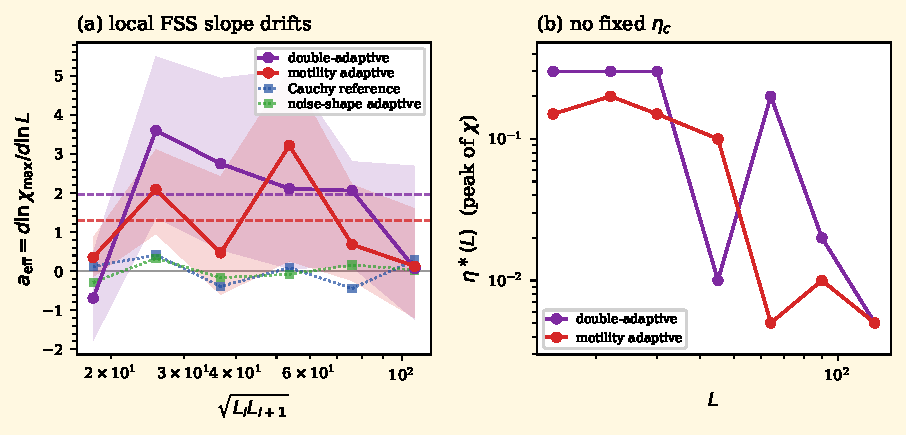
\includegraphics[width=\linewidth]{fig_double_collapse.pdf}
    \caption{Finite-size-scaling diagnostic on the homogeneous
    ten-seed series. (a) local effective slope
    $a_{\rm eff} = d\ln\chi_{\max}/d\ln L$ between consecutive
    sizes, plotted at the geometric-mean size; dashed lines mark
    each mode's global log--log fit. The two motility-active
    modes overshoot their global slope at intermediate $L$ and
    collapse toward zero in the largest interval, whereas the
    Cauchy and noise-shape references hug $a_{\rm eff}\simeq0$
    throughout; bands are $95\%$ seed bootstraps ($B=4000$). (b)
    position $\eta^\ast(L)$ of the susceptibility peak: instead of
    converging to a size-independent $\eta_c$, it migrates toward
    the small-$\eta$ boundary, so the scaling variable
    $(\eta-\eta_c)L^{1/\nu}$ of a standard collapse cannot be
    defined here.}
    \label{fig:collapse}
\end{figure}

A standard collapse $\chi/L^{a}$ against
$(\eta-\eta_c)L^{1/\nu}$ needs a size-independent critical point
$\eta_c$. Panel (b) shows there is none: the susceptibility peak
$\eta^\ast(L)$ does not settle but drifts toward the smallest
accessible noise as $L$ grows, the signature of an
order-from-density (MIPS-like) growth in which $\chi$ keeps
rising as $\eta \to 0$ rather than diverging at a finite
$\eta_c$. With the slope still drifting and the peak still
migrating, we report $a_{\rm full}$ and
$a_{\rm motility}$ as the growth rate of a finite-size
phase-separation susceptibility, and the each-own-$\eta$ excess
($\Delta_7 = +0.63$ on the seven-size sub-grid, $\Delta_9 = +0.45$
across all nine sizes) as a finite-size crossover gap rather than
a difference of asymptotic exponents. The matched-noise control
of the main text shows even this excess is a dense-noise effect:
retuning motility-only to the full mode's dense decorrelation
collapses it to $\Delta_9 = +0.02$.

\end{document}
